\documentclass[a4paper,12pt]{article}

\input{tools/packages.tex}
\input{tools/styles.tex}
\input{tools/acro.tex}

\begin{document}

%%% COVER %%%
\fancypagestyle{alim}{\fancyhf{}\renewcommand{\headrulewidth}{0pt}
\cfoot{
\includegraphics[height=2.2cm]{img/logos/logo_telecos.png}}
}
\thispagestyle{empty}
\begin{center}
{\sffamily 
\resizebox{0.8\textwidth}{!}{
\includegraphics{img/logos/upc_completo+telecos.png}}\\
\vspace{1cm}
{\Huge Deep Learning for Neurodegenerative Disease detection through Spontaneous Speech}\\
\vspace{0.5cm}
{\color{black}\rule{\linewidth}{1pt}}
\vspace{1cm}
{\large{Master Thesis\\
submitted to the Faculty of the \\
Escola T\`ecnica d'Enginyeria de Telecomunicaci\'o de Barcelona \\
Universitat Polit\`ecnica de Catalunya \\
by\\
\vspace{0.4cm}
Roger Esteve}}

\vspace{1.5cm}

{In partial fulfillment\\
of the requirements for the master in\\
\textit{Master’s degree in Advanced Telecommunication Technologies (MATT), track in
Deep Learning for Multimedia Processing}}

\vspace{2cm}

{{Advisor: Dr Francisco Javier Hernando Pericas}} \\
{{Barcelona, June 2026}}
\thispagestyle{alim}
}

%%% INDEX %%%
\end{center}
\newpage
\tableofcontents

%%% LISTS %%%
\newpage
\listoffigures
\lstlistoflistings
\listoftables

%%% REVISION %%%
\newpage
%\input{revision_history}

%%% ABSTRACT %%%
\clearpage
\newpage
\section*{Abstract}

Speech is an attractive non-invasive biomarker for neurodegenerative disease, but multimodal systems that combine acoustic and textual signals expose many interacting design choices whose individual contributions are rarely isolated. This thesis treats such a system as a composition of largely independent design axes (modality, fusion, audio--text alignment, Wav2Vec layer pooling, layer mixing, and feature extractor) and estimates the contribution of each through controlled ablations across three clinical tasks: Alzheimer's disease classification on ADReSSo, amyloid-$\beta$ status prediction, and primary progressive aphasia variant classification. Its central methodological contribution is a pair of token-to-token alignment schemes, uniform and proportional, that refine the word-to-token alignment of prior work at the subword level. The strongest per-axis choices are consolidated into a single configuration-driven implementation, yielding a recommended architecture that is competitive across tasks while remaining lightweight and deployable.

\clearpage
\newpage
\section{Introduction}

Alzheimer's disease is the most common cause of dementia worldwide and is driven by the progressive accumulation of amyloid-$\beta$ plaques and neurofibrillary tau tangles, a pathological process that begins years before clinical symptoms become apparent~\cite{hardy1992amyloid}.
Identifying individuals who harbour this pathology early is a central goal of current research, yet confirmatory assessment still relies on cerebrospinal fluid assays or molecular neuroimaging, procedures that are expensive, invasive, or capacity constrained.
At the syndrome level, primary progressive aphasia (PPA) presents additional diagnostic challenges: three canonical variants are recognised (non-fluent/agrammatic, semantic, and logopenic)~\cite{gorno2011ppa,gorno2015ppa}, but behavioural overlap between them makes clinical differentiation difficult, particularly in early or atypical presentations~\cite{elahi2017clinicopath}.
Both the need for scalable amyloid screening and the challenge of PPA subtyping motivate the development of non-invasive computational tools that can complement expert judgment.

Spontaneous speech is an attractive candidate for this purpose because it simultaneously engages cognitive planning, lexical access, syntactic construction, motor execution, and prosodic control, all of which may be differentially affected by neurodegenerative pathology.
Compared to imaging or fluid biomarkers, voice can be acquired frequently, remotely, and at low marginal cost~\cite{rezaii2025voiceprints}.
Structured elicitation tasks such as the Cookie Theft picture description from the Western Aphasia Battery~\cite{kertesz1982wab} are already part of routine neuropsychological batteries, and recordings from these tasks can be processed computationally without additional clinical instrumentation.

Early computational approaches to cognitive assessment from speech relied on handcrafted linguistic descriptors and shallow acoustic statistics, demonstrating feasibility but limited generalisation~\cite{fraser2016linguistic}.
The shift toward deep learning, particularly self-supervised speech encoders such as wav2vec~2.0~\cite{baevski2020wav2vec} and contextual text models from the BERT family~\cite{devlin2019bert}, has substantially improved representational capacity.
Community benchmarks such as the ADReSSo challenge~\cite{luz2021adresso} have enabled systematic comparison under controlled conditions, and surveys of this literature consistently report that multimodal systems combining acoustic and textual information outperform either modality alone~\cite{ding2024speechsurvey}.

Despite this progress, most published pipelines report end-to-end accuracy figures that conflate several design choices simultaneously: the modality mix, the fusion architecture, the strategy for aligning acoustic frames with text tokens, and the configuration of the self-supervised encoder.
Because these choices are typically entangled within a single system, it is difficult to determine which technique drives the observed performance and which is incidental to the particular implementation or dataset.
Furthermore, the majority of benchmarked systems target English corpora, and it is unclear how well observed trends transfer to languages with different morphology and prosodic norms.
Spanish-speaking clinical cohorts with pathology-confirmed labels exist through initiatives like the Sant Pau Initiative on Neurodegeneration (SPIN)~\cite{alcolea2019spin}, but these have received limited attention in the multimodal deep learning literature.

\subsection{Motivation and objectives}

This thesis is motivated by the observation that, although multimodal speech-based systems for cognitive assessment have shown promising results, the field lacks a systematic understanding of which individual design choices drive performance.
Published systems vary simultaneously in modality, fusion mechanism, audio-text alignment strategy, and encoder configuration, making it impossible to attribute gains to any single technique.
A structured ablation programme, in which each axis is varied while the others are held at controlled defaults, is needed to disentangle these contributions and guide future system design.

Preliminary investigations into deep learning approaches for AD and PPA classification on the ADReSSo and SPIN cohorts were reported in a companion study~\cite{esteve2025speechadppa}; the present thesis extends that work by decomposing the pipeline into individually ablatable design choices.
The main objectives of this thesis are:

\begin{enumerate}
    \item Quantify the individual and combined contribution of audio, text, and handcrafted acoustic features across three clinical speech tasks: AD classification (ADReSSo, English), amyloid-$\beta$ status prediction (SPIN, Spanish), and PPA variant classification (WAB, Spanish).
    \item Systematically compare seven sequence-to-sequence fusion architectures (self-attention, multi-head self-attention, transformer with positional encoding, cross-attention, gated cross-attention, bidirectional cross-attention, and Mamba), evaluated on all three tasks and replicated across two independent implementations.
    \item Propose and evaluate two novel token-to-token audio-text alignment schemes (uniform and proportional) that operate at the subword level, benchmarked against the word-to-token alignment of CogniAlign~\cite{ortiz2025cognialign}.
    \item Evaluate final-layer versus weighted multi-layer Wav2Vec pooling strategies, replicated across both codebases.
    \item Synthesise the experimental evidence into a recommended hybrid architecture that combines the strongest techniques identified along each ablation axis.
\end{enumerate}

\subsection{Work plan}
\label{ssec:workplan}

% TODO: Update gantt_diagrama.tex with actual project phases and dates.
% The current file contains template data from 2019–2020 that must be replaced
% with the real thesis timeline (literature review, implementation, experiments,
% writing phases, milestones, and defence date).

\begin{figure}[H]
    \centering
    \resizebox{\textwidth}{!}{%
\begin{ganttchart}[y unit title=0.4cm,
y unit chart=0.5cm,
vgrid,hgrid,
title height=1,
today=19,%
today offset=.5,%
today label=Now,%
bar/.style={draw,fill=cyan},
bar incomplete/.append style={fill=yellow!50},
bar height=0.7]{1}{20}

 % months (Feb--Jun 2026), four weeks each
 \gantttitle{Master Thesis (February--June 2026)}{20} \\
 \gantttitle{February}{4}
 \gantttitle{March}{4}
 \gantttitle{April}{4}
 \gantttitle{May}{4}
 \gantttitle{June}{4} \\

 % --- Background & data ---
 \ganttgroup[inline=false]{Background \& data}{1}{8}\\
 \ganttbar[progress=100,name=lit]{Literature review}{1}{5} \\
 \ganttbar[progress=100,name=prep]{Data preprocessing \& embedding cache}{2}{8} \\

 % --- Modelling & experiments ---
 \ganttgroup[inline=false]{Modelling \& experiments}{5}{16}\\
 \ganttbar[progress=100,name=prim]{Primitive stacks (CogniAligned, SER)}{5}{10} \\
 \ganttbar[progress=100,name=abl]{Fusion / pooling / alignment ablations}{8}{12} \\
 \ganttbar[progress=100,name=res]{Unified \texttt{res\_model} implementation}{11}{15} \\
 \ganttbar[progress=90,name=mix]{Layer-mixer \& encoder ablations}{13}{16} \\

 % --- Synthesis & writing ---
 \ganttgroup[inline=false]{Synthesis \& writing}{14}{20}\\
 \ganttbar[progress=85,name=ana]{Results analysis}{15}{18} \\
 \ganttbar[progress=65,name=wri]{Thesis writing}{14}{20} \\
 \ganttbar[progress=0,name=def]{Defence preparation}{19}{20} \\

 % dependencies
 \ganttlink{prep}{prim}
 \ganttlink{prim}{abl}
 \ganttlink{abl}{res}
 \ganttlink{res}{mix}
 \ganttlink{mix}{ana}
 \ganttlink{ana}{wri}
 \ganttlink{wri}{def}

\end{ganttchart}%
}

    \caption{Gantt diagram of the project.}
    \label{fig:gantt}
\end{figure}


%%% StateOfTheArt %%%
\clearpage\section{State of the art of the technology used or applied in this thesis}
\label{sec:sota}

This chapter surveys the scientific and technical background that motivates analysis of spontaneous speech with deep multimodal models in neurodegenerative disease.
The discussion follows the structure of recent surveys and challenge-led benchmarking in speech-based cognitive assessment~\cite{ding2024speechsurvey}, but it is organised around the specific threads that underpin the companion contribution developed in this thesis~\cite{esteve2025speechadppa}: pathology-aware biomarker estimation from voice, differential diagnosis of primary progressive aphasia (PPA), cross-lingual dataset gaps, self-supervised acoustic encoders paired with language-model text encoders, fusion architectures that align modalities in time, and the complementary role of handcrafted paralinguistic descriptors.
Throughout, emphasis is placed on results and modelling trends that are reproducible on public benchmarks---notably the Alzheimer's Dementia Recognition through Spontaneous Speech Only (\textsc{ADReSS}o) corpus associated with the challenge formulation of Luz et al.~\cite{luz2021adresso}---and on how those trends inform deployment on clinically curated cohorts such as the Sant Pau Initiative on Neurodegeneration (SPIN)~\cite{alcolea2019spin}.

\subsection{Biological motivation: amyloid pathology and clinically overlapping syndromes}

Accumulation of amyloid-$\beta$ (\textsc{A}$\beta$) is a core pathophysiological substrate in Alzheimer's disease (AD) research and underpins current therapeutic strategies that lean on early biological identification of at-risk individuals~\cite{hardy1992amyloid}.
Confirmatory assessment traditionally relies on cerebrospinal fluid assays or molecular neuroimaging; although accurate, these modalities are expensive, invasive, or capacity constrained, which contributes to delayed detection relative to symptom onset and limits scalable screening in population settings.

Parallel to biomarker science, differential diagnosis at the syndrome level remains difficult because language and executive deficits arise across neurodegenerative aetiologies with partially overlapping phenotypes.
PPA exemplifies this tension: it is defined as a progressive disorder of language as the principal complaint and functional limitation, and contemporary consensus schemes stratify variants according to the dominant cognitive-linguistic profile~\cite{gorno2011ppa,gorno2015ppa}.
The non-fluent/agrammatic (\textit{nfv}), semantic (\textit{sv}), and logopenic (\textit{lv}) variants differ in fluency, grammatical competence, lexical--semantic knowledge, and repetition/spelling-span signatures; importantly, variant labels provide clinically actionable hypotheses about underlying proteinopathy patterns even though symptoms can blur across boundaries~\cite{elahi2017clinicopath}.
From an engineering viewpoint, these clinical facts motivate pattern recognition systems that are sensitive to subtle temporal micro-structure of speech (planning pauses, articulatory slowing, reduced informational density) and to lexical--semantic content jointly---precisely the multimodal cues accessible from spontaneous picture descriptions or narrative tasks collected during routine assessments~\cite{lima2025communicationsmedicine}.

\subsection{Spoken language as a scalable digital biomarker}

Prospective clinicopathological studies and controlled biomarker programmes increasingly incorporate speech and language markers alongside imaging and fluid assays because voice can be acquired frequently, remotely, and at comparatively low marginal cost~\cite{rezaii2025voiceprints}.
At the same time, evaluation methodology matters: speech measures can track syndrome severity and risk enrichment, yet population heterogeneity (education, dialect, comorbid hearing loss, task instructions) can inflate apparent effects unless modelling assumptions are carefully matched to sampling designs~\cite{lima2025communicationsmedicine}.

Early computational work emphasised engineered linguistic descriptors extracted from transcripts (lexical diversity, syntactic complexity, idea density) and shallow acoustic statistics computed from short recordings of spontaneous speech to separate AD from healthy ageing~\cite{fraser2016linguistic}.
These approaches demonstrated feasibility but often relied on manual transcription pipelines or handcrafted feature dictionaries whose coverage is incomplete for noisy clinical audio.
More recent analyses revisit classical machine-learning baselines (random forests, support-vector machines) with richer descriptors and report uneven sensitivity depending on task elicitation and recording conditions~\cite{lima2025communicationsmedicine}; collectively, such studies argue that marker families carry predictive signal but that shallow decision boundaries under-use temporal dynamics present in the waveform~\cite{fristed2022leveraging,gabirondo2025speechbiomarkers,slegers2021connectedppa}.

\subsection{From shallow classifiers to deep neural representations}

Representation learning replaces brittle front-ends with hierarchical embeddings trained either supervised end-to-end or semi-supervised with objectives aligned to phonetic/lexical structure.
In speech processing broadly, self-supervised pre-training of transformer acoustic models (wav2vec~2.0~\cite{baevski2020wav2vec}, HuBERT~\cite{hsu2021hubert}, WavLM~\cite{chen2022wavlm}) learns frame-level features transferable across languages and domains with comparatively modest labelled downstream data.
Parallel advances in text modelling yield contextual token embeddings (BERT family~\cite{devlin2019bert}; lighter distilled variants such as DistilBERT~\cite{sanh2019distilbert}; modern long-context encoder-only architectures such as ModernBERT~\cite{warner2025modernbert}) that capture lexical semantics and local syntax when transcript hypotheses are available.

Reviews oriented specifically at AD detection from speech highlight two robust tendencies~\cite{ding2024speechsurvey}: deep neural pipelines dominate leaderboard-style benchmarks when adequate training partitions exist, and multimodal systems that consume both acoustic embeddings and text outperform either modality alone when transcripts are informative enough for alignment~\cite{ding2024speechsurvey}.
These observations motivate architectures that treat spontaneous speech as \emph{tightly coupled} audio--text sequences rather than as isolated vectors~\cite{macoir2025rethinkingppa}.

\subsection{Benchmark challenges and public corpora}

Community challenges accelerated reproducible comparison by freezing splits and evaluation protocols for cognitive impairment detection from speech-only submissions~\cite{luz2021adresso}.
The \textsc{ADReSS}o subset derived from the DementiaBank Pitt corpus of picture descriptions remains the de facto English benchmark for Alzheimer's dementia versus healthy control discrimination under matched recording conditions; numerous challenge systems established competitive baselines~\cite{syed2021muetrmit}, and subsequent work continues to extend feature attribution and model explanations~\cite{ntampakis2025neuroxvocal}.

However, performance on English benchmarks does not trivially transfer to other languages: morphology, prosodic norms, and clinician elicitation protocols differ, and labelled neurodegeneration cohorts at scale remain comparatively scarce outside a handful of reference centres.
Initiatives such as SPIN address biomarker discovery and validation by assembling multicentre observational data spanning genetics, imaging, fluid markers, and structured cognitive assessments~\cite{alcolea2019spin}; subsets incorporating spontaneous speech tasks tied to standard batteries (for example picture-description prompts compatible with the Western Aphasia Battery~\cite{kertesz1982wab}) enable language-specific baselines that complement English challenge corpora.

Spanish-focused clinical studies demonstrate that machine-learning models incorporating language-aware descriptors can achieve strong discrimination between PPA variants~\cite{matias2019machineppa}, while recent bilingual analyses underscore that acoustic models may retain utility even when patients produce speech in a non-dominant language, whereas lexical models become comparatively brittle---a caution for multimodal pipelines deployed in multilingual clinics~\cite{pugalenthi2024bilingualppa}.

\subsection{Automatic differentiation of PPA variants from connected speech}

Because syndromic overlap complicates visual inspection alone, quantitative speech analyses seek markers that track breakdown profiles hypothesised by neurolinguistic models: reduced speech rate and grammatical complexity in \textit{nfvPPA}; lexical retrieval failures and semantic thinning in \textit{svPPA}; hesitation and phonological loop limitations with spared grammar in \textit{lvPPA}~\cite{gorno2011ppa}.

Empirical studies highlight pause structure, filler usage, lexical diversity, and discourse coherence metrics as discriminative at group level~\cite{cho2022lexical}, while articulatory tempo measures help separate non-fluent from fluent variants~\cite{cordella2017articulation,haley2021speechmetrics}.
At the intersection with amyloid biology, connected speech features associate with cortical amyloid burden within PPA cohorts~\cite{slegers2021connectedppa}, reinforcing the notion that speech captures not only syndrome labels but correlates of underlying pathology---similar in spirit to speech-only screening models targeting amyloid positivity~\cite{fristed2022leveraging,gabirondo2025speechbiomarkers}.

Recent proof-of-concept studies escalate modelling complexity: large language models combined with curated linguistic measurements attain high classification accuracy in retrospective cohorts~\cite{rezaii2024ppallm}, whereas neural architectures trained jointly on acoustic and linguistic embeddings yield competitive multi-class accuracy relative to expert benchmarks~\cite{themistocleous2021automatic}.
Nevertheless, models remain sensitive to sample size and label noise; moreover, cross-cohort validation across accents and tasks remains an open engineering constraint~\cite{nevler2019validated}.

\subsection{Multimodal fusion: pooling, cross-attention, and temporal alignment}

Multimodal classifiers must reconcile wildly different sampling rates: acoustic frames at millisecond resolution versus word or sub-word tokens at comparatively coarse timestamps derived from automatic speech recognition~\cite{ding2024speechsurvey}.
Early fusion concatenates embeddings after temporal pooling; intermediate fusion stacks modalities into sequences processed by self-attention (multi-head attention pooling aggregates variable-length sequences into fixed vectors); late fusion retains modality-specific encoders until decision layers~\cite{esteve2025speechadppa}.

Orthogonal to pooling choices, \emph{cross-modal alignment} seeks to reduce leakage between mis-synchronised streams---for instance when silences precede lexical onsets or when patients produce lengthened syllables spanning multiple phones~\cite{ortiz2025cognialign}.
The CogniAlign architecture exemplifies word-level alignment between acoustic frames and textual tokens before gated cross-attention refinement~\cite{ortiz2025cognialign}; intuitively, synchronisation encourages the network to allocate attention to co-occurring acoustic evidence (jitter, spectral tilt shifts, lengthened closures) and lexical hypotheses rather than to incidental nuisance correlates.

Independent multimodal systems repurposed from speaker and emotion modelling demonstrate that competitive fusion architectures transfer across paralinguistic tasks when augmented with domain regularisation~\cite{naini2025interspeechser}; this lineage motivates evaluating robust encoder stacks originally optimised on emotion corpora when ported to clinical speech~\cite{esteve2025speechadppa}.

\subsection{Handcrafted acoustic descriptors alongside learned embeddings}

Despite the strength of self-supervised waveform encoders, clinically interpretable descriptors remain attractive because they tie predictions to measurable articulatory and phonatory parameters (pause histograms, intensity envelopes, fundamental-frequency variation, shimmer/jitter, harmonics-to-noise ratio, spectral moments, formant tracks, cepstral coefficients).
Pause-oriented statistics repeatedly emerge as salient in cognitive decline~\cite{imre2022temporal,zheng2024survey}; voice-quality perturbations may track neurogenic speech motor control deficits~\cite{rezaii2025voiceprints}.

Open-source dementia-speech pipelines demonstrate competitive accuracy when coupling classical descriptors with modern backbones~\cite{ntampakis2025neuroxvocal}, supporting hybrid designs where auxiliary vectors augment attention pooling or concatenate immediately before classification~\cite{esteve2025speechadppa}.
Whether explicit features complement latent embeddings in practice depends on architecture and task: pathology-linked cues sometimes persist outside generic waveform embeddings, whereas architectures with explicit alignment may subsume part of the prosodic signal~\cite{ortiz2025cognialign}.

\subsection{Synthesis and positioning}

Taken together, the literature supports three design commitments reflected in the methodological arc of this thesis~\cite{esteve2025speechadppa}: \emph{(i)} evaluate pathology-aware models where biology-grounded labels exist (for example \textsc{A}$\beta$ status alongside syndrome diagnoses), not solely dementia-vs-control proxies; \emph{(ii)} benchmark competing multimodal fusion philosophies using harmonised preprocessing on both an English reference corpus (\textsc{ADReSS}o) and a clinically curated Spanish-speaking subset aligned with SPIN; and \emph{(iii)} quantify when handcrafted acoustic descriptors remain complementary after state-of-the-art self-supervised acoustic encoding and explicit audio--text alignment~\cite{ding2024speechsurvey,ortiz2025cognialign,ntampakis2025neuroxvocal}.

The following methodology chapter translates these commitments into concrete architectures, training protocols, and evaluation choices.


%%% METHODOLOGY %%%
\clearpage\section{Methodology and Project Development}
\label{sec:methodology}

\subsection{Problem Formulation}
\label{ssec:problem_formulation}

The general problem addressed in this thesis is the prediction of a clinical label from a single recording of spontaneous speech elicited by a structured picture-description task. Each sample is a pair $(x^{\mathrm{a}}, x^{\mathrm{t}})$, where $x^{\mathrm{a}}$ is the raw acoustic waveform and $x^{\mathrm{t}}$ is the corresponding transcript of the utterance, and the goal is to learn a mapping $f_\theta : (x^{\mathrm{a}}, x^{\mathrm{t}}) \mapsto y$, where $y \in \mathcal{Y}$ is a discrete diagnostic label whose domain depends on the task.

We study three tasks, each defined over a distinct clinical cohort and summarised in Table~\ref{tab:datasets}. The first is Alzheimer's disease classification, a binary discrimination between AD patients and cognitively normal (CN) controls on the English ADReSSo cohort~\cite{luz2021adresso}, with $\mathcal{Y} = \{\mathrm{AD}, \mathrm{CN}\}$; this is the only task with an official held-out test partition. The second is amyloid-$\beta$ status prediction, a binary proxy-biomarker task defined on a Spanish-speaking subset of the SPIN cohort~\cite{alcolea2019spin} elicited with the Western Aphasia Battery picture-description task~\cite{kertesz1982wab}, with $\mathcal{Y} = \{\mathrm{positive}, \mathrm{negative}\}$. The third is primary progressive aphasia variant classification, a three-class problem distinguishing the non-fluent/agrammatic, semantic, and logopenic variants~\cite{gorno2011ppa} defined on the same SPIN subset, with $|\mathcal{Y}| = 3$. Both Spanish tasks are drawn from this single SPIN subset and share the same data tree; neither has an official external test split, so for these we report cross-validated performance only and never construct an artificial test partition.

Both modalities are encoded by frozen self-supervised models. The acoustic stream is processed by a Wav2Vec~2.0 encoder~\cite{baevski2020wav2vec} (the specific variant depends on the implementation and is detailed in Section~\ref{ssec:architecture}) producing a frame-level sequence $\mathbf{H}^{\mathrm{a}} = (\mathbf{h}^{\mathrm{a}}_1, \dots, \mathbf{h}^{\mathrm{a}}_{T_a})$, and the textual stream by a frozen transformer text encoder of the BERT family~\cite{devlin2019bert}, producing a token-level sequence $\mathbf{H}^{\mathrm{t}} = (\mathbf{h}^{\mathrm{t}}_1, \dots, \mathbf{h}^{\mathrm{t}}_{T_t})$. Because the two sequences live on different time bases ($T_a \neq T_t$), an alignment step is required to place acoustic and textual representations on a common index before they can be fused, after which a sequence-to-sequence fusion module combines the aligned streams into a representation that feeds a shallow classification head.

Rather than treating this pipeline as a single monolithic system optimised end to end, this thesis formulates it as the composition of six largely independent design axes, each of which can be varied while the others are held at controlled defaults. The modality axis $m$ determines whether the classifier consumes audio alone, text alone, their combination, or additionally a set of handcrafted acoustic features. The fusion axis $f$ selects the sequence-to-sequence architecture that combines the aligned acoustic and textual streams, drawn from a catalogue of seven families. The alignment axis $a$ fixes the scheme that maps acoustic frames onto text positions, comprising the word-to-token baseline of CogniAlign~\cite{ortiz2025cognialign} and the two token-to-token schemes proposed in this work. The Wav2Vec pooling axis $w$ chooses between the final encoder layer and a learnable weighted sum across layers. The layer-mixing axis $\ell$ refines that choice: in place of a single global set of layer weights, an adaptive mixer can learn to combine the encoder's layers per utterance, or even per token, so that the depth of representation is selected dynamically rather than fixed in advance. Finally, the feature-extractor axis $e$ varies the pretrained encoders themselves, substituting one audio or text backbone for another, to test how far the downstream trends depend on the specific self-supervised models that supply the two streams.

A concrete system instance is thus parameterised by a tuple $(m, f, a, w, \ell, e)$, and the central empirical question is to estimate the marginal contribution of each axis, alone and in interaction, on the three tasks, rather than to identify a single best-performing run. The unit of comparison is therefore the \emph{technique}, not the implementation: two independent codebases replicate the fusion and Wav2Vec-pooling trends under a second software stack, and a third, configuration-unified implementation then consolidates the resulting techniques into a single model (Section~\ref{ssec:architecture}). Building on this decomposition, the experimental programme of Section~\ref{sec:experiments} traverses the axes in a staged sequence, and the synthesis of the strongest choice along each axis into a recommended hybrid architecture is taken up in the Discussion.

\subsection{Datasets and Preprocessing}
\label{ssec:datasets}

The three tasks defined in Section~\ref{ssec:problem_formulation} are evaluated on two clinical cohorts, summarised in Table~\ref{tab:datasets}: the English ADReSSo benchmark for AD classification, and a curated subset of the Spanish-speaking SPIN cohort that supplies both the amyloid-$\beta$ and PPA tasks. They differ in language, label space, and the availability of a held-out test partition, which in turn governs the evaluation protocol applied to each (Section~\ref{ssec:evaluation}). All recordings originate from structured picture-description tasks, so the input distribution is comparable across cohorts even though the underlying populations and elicitation languages differ. The cohort descriptions and demographic characterisation below follow the companion paper in which we first introduced this SPIN subset~\cite{esteve2025speechadppa}; the remainder of the subsection details each cohort and the common preprocessing pipeline that turns raw recordings into the paired acoustic and textual representations consumed by the model.

\begin{table}[H]
\centering
\caption[Clinical cohorts and evaluation protocol]{\footnotesize Clinical cohorts, languages, label spaces, and evaluation protocol. Only the English ADReSSo cohort provides an official held-out test partition; the two Spanish tasks are evaluated by stratified cross-validation. Both Spanish tasks are drawn from the same SPIN subset, elicited with the Western Aphasia Battery picture-description (``Picnic Scene'') task.}
\label{tab:datasets}
\footnotesize{
\begin{tabular}{@{}llccl@{}}
\toprule
\textbf{Task} & \textbf{Cohort} & \textbf{Language} & \textbf{Classes} & \textbf{Evaluation} \\ \midrule
AD vs.\ CN & ADReSSo & English & 2 & Official \texttt{test-dist} (\texttt{test\_acc}) \\
Amyloid-$\beta$ status & SPIN & Spanish & 2 & 5-fold CV (validation only) \\
PPA variant & SPIN & Spanish & 3 & 5-fold CV (validation only) \\
\bottomrule
\end{tabular}
}
\end{table}

\subsubsection{ADReSSo Corpus}

The Alzheimer's disease task uses the ADReSSo-IS2021 corpus introduced for the corresponding Interspeech challenge~\cite{luz2021adresso}. The corpus is derived from the English-language DementiaBank Pitt Corpus and comprises 237 spontaneous picture-description recordings, totalling approximately 166 minutes of speech, in which participants describe the Cookie Theft scene from the Boston Diagnostic Aphasia Examination. It is balanced between AD patients and healthy controls and matched for age and sex, which removes the most obvious demographic confounds and makes it a clean benchmark for isolating speech-based effects. The challenge distributes a fixed train and \texttt{test-dist} split, so this is the only task in the thesis with an official external test set and therefore the only one on which we report a held-out test accuracy in addition to cross-validated performance. We use ADReSSo primarily to anchor the architecture against a well-documented English benchmark, as in our companion paper~\cite{esteve2025speechadppa}, rather than to optimise exhaustively for the challenge leaderboard.

\subsubsection{SPIN Clinical Cohort}

The two Spanish tasks are defined on a curated subset of the Sant Pau Initiative on Neurodegeneration (SPIN)~\cite{alcolea2019spin}, a longitudinal cohort for biomarker discovery and validation in neurodegenerative disorders maintained at the Hospital de la Santa Creu i Sant Pau in Barcelona. From this cohort we assembled a set of Spanish-speaking participants for whom spontaneous speech recordings, a confirmed amyloid-$\beta$ status, and, where applicable, a clinical PPA variant diagnosis were all available~\cite{esteve2025speechadppa}. Unlike ADReSSo, the elicitation stimulus is the ``Picnic Scene'' from the Western Aphasia Battery~\cite{kertesz1982wab}, and recordings were captured during routine clinical evaluations, with a variable number of samples per subject ranging from one to seven. This repeated-measures structure is the reason all cross-validation on SPIN is stratified by subject identifier, so that recordings from the same participant never straddle the train and validation folds; reporting at the recording level rather than the subject level would otherwise leak speaker identity and inflate the estimated accuracy.

The subset supports two clinically distinct tasks. The amyloid-$\beta$ prediction task is a binary problem that asks the model to predict amyloid positivity, a fluid biomarker of AD whose confirmation otherwise requires costly or invasive cerebrospinal-fluid assays or PET imaging. At the subject level it comprises 53 amyloid-positive and 49 amyloid-negative participants, and at the recording level 114 positive and 98 negative samples, leaving the task approximately balanced. The PPA variant classification task is a three-class problem distinguishing the logopenic (lvPPA), non-fluent/agrammatic (nfvPPA), and semantic (svPPA) variants, with 35, 22, and 17 subjects and 104, 63, and 35 recordings respectively. This task is markedly imbalanced (svPPA accounts for fewer than a third of the lvPPA recordings), and the small per-class subject counts make fold-level performance estimates high-variance, so the PPA results are interpreted with corresponding caution.

Tables~\ref{tab:demo_amyloid} and~\ref{tab:demo_ppa} report the demographic composition of the two tasks. No statistically significant differences in age, sex, or years of education were found across the groups of either task, assessed with the Wilcoxon rank-sum test for continuous variables and Pearson's chi-squared test for categorical ones~\cite{esteve2025speechadppa}; this matching is important because it makes it less likely that a classifier exploits demographic shortcuts rather than disease-related speech characteristics.

\begin{table}[H]
\centering
\caption[SPIN demographics by amyloid status]{\footnotesize Demographic composition of the SPIN amyloid-$\beta$ task by subject. Values are mean\,$\pm$\,SD or $n$ (\%).}
\label{tab:demo_amyloid}
\footnotesize{
\begin{tabular}{@{}lcc@{}}
\toprule
 & \textbf{Negative} ($N=49$) & \textbf{Positive} ($N=53$) \\ \midrule
Age (years)      & $72.8\pm6.1$ & $72.6\pm6.8$ \\
Female           & $25$ ($51.0\%$) & $22$ ($41.5\%$) \\
Male             & $24$ ($49.0\%$) & $31$ ($58.5\%$) \\
Education (years)& $12.8\pm6.6$ & $11.8\pm5.7$ \\
\bottomrule
\end{tabular}
}
\end{table}

\begin{table}[H]
\centering
\caption[SPIN demographics by PPA variant]{\footnotesize Demographic composition of the SPIN PPA task by subject. Values are mean\,$\pm$\,SD or $n$ (\%).}
\label{tab:demo_ppa}
\footnotesize{
\begin{tabular}{@{}lccc@{}}
\toprule
 & \textbf{lvPPA} ($N=35$) & \textbf{nfvPPA} ($N=22$) & \textbf{svPPA} ($N=17$) \\ \midrule
Age (years)      & $72.6\pm6.5$ & $74.7\pm4.9$ & $73.4\pm5.8$ \\
Female           & $15$ ($42.9\%$) & $9$ ($40.9\%$) & $11$ ($64.7\%$) \\
Male             & $20$ ($57.1\%$) & $13$ ($59.1\%$) & $6$ ($35.3\%$) \\
Education (years)& $10.4\pm6.4$ & $12.6\pm5.9$ & $9.8\pm6.9$ \\
\bottomrule
\end{tabular}
}
\end{table}

\subsubsection{ASR Pipeline and Transcript Quality}

The textual modality is derived from the audio rather than from gold manual transcripts, so that the pipeline reflects a realistic deployment in which only recordings are available. Each recording is first truncated to its initial forty seconds of speech, which approximates the effective input length of the alignment-based model and, on the SPIN data, avoids capturing the clinician speech that occasionally appears toward the end of an evaluation. The truncated audio is then transcribed automatically with Whisper, though the two stacks differ in configuration: the CogniAligned pipeline runs the Whisper \texttt{turbo} model offline to obtain transcripts together with the word-level timestamps its alignment step requires, whereas the SER pipeline reuses precomputed transcripts where they are available and falls back to the lightweight Whisper \texttt{tiny} model otherwise. The resulting transcript is tokenised by the text encoder before being aligned with the acoustic stream. Because recognition errors propagate into the textual representation, transcript quality is a genuine source of variance, particularly for the Spanish cohort and for the disfluent or aphasic speech characteristic of PPA; the experiments therefore treat the text modality as one ablatable input among several rather than as a noise-free signal.

\subsection{System Architecture}
\label{ssec:architecture}

The model follows a two-stream design in which audio and text are embedded independently by frozen self-supervised encoders, aligned onto a common sequence index, combined by a sequence-to-sequence fusion module, and finally pooled and mapped to a task label by a lightweight head (Figure~\ref{fig:system_architecture}). Each stage corresponds to one of the design axes introduced in Section~\ref{ssec:problem_formulation}: the encoders and their pooling fix the acoustic and textual representations, the alignment step determines how the two time bases are reconciled, and the fusion module determines how the aligned streams interact. The ablation programme depends on this separation: a single axis can be changed while the rest of the pipeline stays fixed.

Both encoders are kept frozen throughout. This is a modelling choice, not a computational shortcut: freezing holds the trainable parameter count in the low millions, concentrates learning capacity in the fusion module under study, and reduces the risk of overfitting the small clinical cohorts. It has a practical payoff as well. Once the encoder outputs are deterministic, every embedding can be computed once and cached, and that cache is what makes a multi-axis grid of experiments tractable at all.

The architecture is realised across three complementary implementations. CogniAligned and SER are the two \emph{primitive} stacks in which the individual techniques were developed and ablated: CogniAligned is the full pipeline and the only stack that implements subword token alignment, whereas SER operates on segment-level representations and serves to check whether the fusion and Wav2Vec-pooling trends reproduce under a second, independent implementation. The two stacks differ in their encoders and training schedule, so results are compared across them as directional agreement, not exact reproduction---a caveat that applies wherever cross-stack figures are quoted in what follows. Building on both, \texttt{res\_model} is a third, configuration-driven implementation that consolidates these techniques into a single model: any combination of modality, fusion, alignment, Wav2Vec pooling, layer mixing, and feature extractor is selected from one configuration, so the strongest choices identified separately on the primitive stacks can be assembled and trained together in a controlled way. The primitive stacks carry the main ablation narrative; \texttt{res\_model} folds their findings into the unified model from which the recommended architecture is drawn (detailed below). That model is competitive with the primitive stacks across the three tasks without being uniformly the best on any single one. Its value lies in integration and deployment, not in a higher accuracy ceiling.

\begin{figure}[ht]
\centering
\fbox{\parbox{0.9\linewidth}{\vspace{4cm}\centering\small\textit{[Figure to be added]}\vspace{4cm}}}
\caption{End-to-end architecture used in this thesis: frozen Wav2Vec~2.0 and BERT-family encoders produce acoustic and textual sequences, which are placed on a common index by the alignment step, combined by the sequence-to-sequence fusion module, and mapped to a task label by a lightweight head.}
\label{fig:system_architecture}
\end{figure}

\subsubsection{Acoustic Encoder: Choice and Configuration}
\label{sssec:acoustic_encoder}

Audio is encoded by a frozen Wav2Vec~2.0 model~\cite{baevski2020wav2vec}, but the two stacks use different variants by design. CogniAligned uses the base configuration (\texttt{facebook/wav2vec2-base-960h}): a convolutional feature encoder maps the raw 16\,kHz waveform to latent frames at roughly 20\,ms resolution (about 50 frames per second), which a twelve-layer transformer context network then contextualises into 768-dimensional hidden states. This model has on the order of 95 million parameters and was trained on 960 hours of English read speech (LibriSpeech); it is therefore monolingual, and CogniAligned applies it unchanged to the Spanish cohorts as well. SER instead uses the cross-lingual XLSR-300M variant, a deeper encoder of roughly 300 million parameters whose twenty-four transformer layers produce 1024-dimensional states and which was pretrained on about 436{,}000 hours of unlabelled speech spanning 128 languages. The two audio encoders thus differ in depth, width, capacity, and language coverage---one more axis on which the two stacks are not matched.

\subsubsection{Wav2Vec Pooling and Layer Mixing}
\label{sssec:pooling}

The encoder is used purely as a frozen feature extractor: its weights are never updated, and the frame-level sequence $\mathbf{H}^{\mathrm{a}}$ is read directly from the transformer stack. How that sequence is formed is the Wav2Vec-pooling axis. The default, used as the controlled setting in every phase except the dedicated pooling study, takes the hidden states of the final transformer layer. The alternative learns one scalar weight per layer, normalises the weights with a softmax, and forms the representation as the weighted sum of all layer outputs (twelve layers for the base encoder in CogniAligned, twenty-four for XLSR-300M in SER). This is motivated by the well-documented observation that the layers of a self-supervised speech encoder specialise in different information (lower layers carry phonetic and speaker detail while higher layers carry more abstract content), so a learnable combination can expose cues that any single fixed layer discards. To further regularise training on the limited clinical data, the SER stack additionally applies on-the-fly acoustic data augmentation, including additive noise, reverberation, and speed perturbation, prior to feature extraction.

The weighted sum just described shares a single set of layer weights across every recording. Making that combination learnable has a clear purpose: instead of committing in advance to the final layer, the model decides for itself which layers to read features from, putting weight wherever the task-relevant signal is strongest. In the recommended base configuration the weighting is a learnable softmax over all twelve transformer layers, and over all twenty-four for the deeper XLSR-300M encoder.

The most informative depth, however, need not be the same for every recording. A refinement evaluated in the unified \texttt{res\_model} implementation therefore makes the weighting adaptive, replacing the one fixed vector with a learnable \emph{layer mixer} that forms the softmax over the layer logits conditionally. It comes in three granularities. A \emph{global} mixer keeps one static weighting for all data. A \emph{sample} mixer predicts a separate weighting per utterance, letting an atypical or noisy recording lean on different layers. A \emph{token} mixer goes finer still, mixing the layers independently at each position. A low temperature ($\tau = 0.1$) sharpens the softmax so the mixer settles on a few layers rather than smearing weight across all of them, and its parameters are trained at about ten times the rate of the rest of the head. The sample mixer is the one carried into the recommended configuration: lightweight, input-conditioned, and in practice biased toward the upper layers.

Mechanically, the mixer acts only on the audio branch and only before fusion, collapsing the layer axis into a single vector per time step; the text embeddings never pass through it. The sample mixer obtains its per-utterance weights by mean-pooling each layer over time and passing the result through a small linear scorer followed by the softmax, so the weighting reflects global properties of the recording; the token mixer instead scores every layer at each position, which amounts to a lightweight attention over layers. This layer mixing should not be confused with attention pooling: the mixer reduces the \emph{depth} (layer) axis before fusion, whereas attention pooling would reduce the \emph{time} axis after fusion, and the recommended configuration uses simple mean pooling for the latter.

\subsubsection{Text Encoder: Choice and Configuration}

Text is encoded by a frozen transformer from the BERT family~\cite{devlin2019bert}, which turns the tokenised transcript into a sequence of contextual token-level embeddings $\mathbf{H}^{\mathrm{t}}$. The two implementations again use different members of this family. CogniAligned uses DistilBERT~\cite{sanh2019distilbert}, a six-layer encoder distilled from BERT-base that retains most of its language-understanding capability at roughly half the parameters and inference cost, matching the original CogniAlign design. SER uses ModernBERT-base~\cite{warner2025modernbert}, a more recent encoder of about 149 million parameters trained on the order of two trillion tokens, with a native 8192-token context window, rotary positional embeddings, GeGLU activations, and an alternating local--global attention pattern that makes long-context encoding efficient.

As with the acoustic encoder, the text encoder is frozen and its embeddings are precomputed. Holding it fixed within each stack ensures that the text representation is not a confound when fusion, alignment, or pooling is varied. The two stacks do use different text encoders, so this is yet another axis on which they are not matched.

\subsubsection{Feature-Extractor Stacks}
\label{sssec:feature_extractors}

The choice of pretrained backbone for each stream is itself a design decision rather than a fixed given, and constitutes the feature-extractor axis introduced in Section~\ref{ssec:problem_formulation}. The two primitive stacks already pair different encoders: CogniAligned combines DistilBERT~\cite{sanh2019distilbert} with the English Wav2Vec~2.0 base model, while SER combines ModernBERT~\cite{warner2025modernbert} with the cross-lingual XLSR-300M. These stacks, however, also differ in their ASR, alignment granularity, and training schedule, so reading the gap between them as an encoder comparison would confound the encoder with everything else that varies. A clean comparison requires changing one encoder at a time while holding the rest of the pipeline fixed.

This is what the unified \texttt{res\_model} implementation provides through a single-factor extractor ablation. Against a fixed recipe (bidirectional cross-attention fusion, word-to-token alignment, the weighted Wav2Vec stack with the per-utterance sample layer mixer, and word-timestamped CogniAligned transcripts), one component is swapped per run and every other factor is held constant. On the audio side the base encoder is replaced by XLSR-300M, to test whether a deeper cross-lingual model helps the Spanish cohorts; on the text side DistilBERT is replaced by ModernBERT and by the undistilled BERT-base~\cite{devlin2019bert}, contrasting a lightweight distilled encoder, a recent long-context one, and the original reference. Each variant is run on all three tasks under two random seeds to expose seed sensitivity. The candidates are deliberately drawn from different points of the design space: DistilBERT for its low cost and its role in the original CogniAlign design, ModernBERT for its modern architecture and long context, BERT-base as the undistilled baseline, and the English base versus cross-lingual XLSR audio encoders for the monolingual-versus-multilingual contrast that is most relevant once the same pipeline is applied to Spanish speech. The per-task outcomes, which prove markedly task-dependent, are reported with the experiments.

\subsubsection{Cross-Modal Alignment}
\label{sssec:alignment}

Before the two streams can be fused they must be placed on a common sequence index, because the acoustic sequence is far longer than the token sequence ($T_a \gg T_t$). CogniAligned resolves this by precomputing an aligned tensor in which each text position is paired with a pooled acoustic representation, and the three alignment schemes differ in how acoustic frames are assigned to text positions. The word-to-token baseline, inherited from CogniAlign~\cite{ortiz2025cognialign}, uses the word-level timestamps produced by the ASR step to mean-pool the acoustic frames spanned by each spoken word into a single vector, which is then replicated at every subword token of that word. The two schemes proposed in this thesis operate one level finer, at the subword granularity produced by the text tokeniser. The \emph{uniform} scheme takes the frame span of each word and divides it evenly among the word's subword tokens, so that a word split into three tokens contributes three equal slices. The \emph{proportional} scheme instead divides the span in proportion to the character length of each subword token, on the assumption that longer subwords tend to occupy more of the spoken word and should therefore receive proportionally more acoustic frames. Both subword schemes yield a finer-grained audio--text correspondence than the word-level baseline, and the comparison among the three constitutes the alignment axis (Figure~\ref{fig:alignment_schemes}). SER does not align at the subword level: it fuses segment-level representations and therefore takes no part in the alignment ablation.

\begin{figure}[ht]
\centering
\fbox{\parbox{0.9\linewidth}{\vspace{4cm}\centering\small\textit{[Figure to be added]}\vspace{4cm}}}
\caption{Audio--text alignment schemes compared in this thesis: the CogniAlign word-to-token baseline, and the two proposed token-to-token schemes (uniform, which spreads each word's frames evenly across its subword tokens, and proportional, which allocates frames to tokens in proportion to their character length).}
\label{fig:alignment_schemes}
\end{figure}

\subsubsection{Fusion Module}

Once the streams are aligned (or, in SER, taken at the segment level), the fusion module combines them into the joint representation that the head consumes. This is the axis the thesis varies most widely. Seven families are implemented and compared, summarised in Table~\ref{tab:fusion}, and they fall into three groups (Figures~\ref{fig:self_attention_fusion}--\ref{fig:mamba_fusion}) that embody three distinct hypotheses about how acoustic and textual evidence ought to interact.

The first group applies \textbf{self-attention} to the concatenated audio--text sequence, treating both modalities as one undifferentiated set of tokens in which every position may attend to every other. Its premise is that the relevant cross-modal structure will surface on its own once the model is given global context, with no architectural separation between the streams. Three variants probe how much machinery that premise actually needs. Plain self-attention uses a single attention map. Multi-head self-attention splits the computation into several parallel heads, each free to specialise in a different relation, one head might track how prosody aligns with content words while another tracks how pauses fall around syntactic boundaries. The transformer-with-positional-encoding variant goes further and injects sinusoidal position information inside a full transformer block~\cite{vaswani2017attention}, so that the order of frames and tokens is modelled explicitly. That last addition matters for speech in particular, where timing is itself diagnostic and a permutation-invariant model would throw away exactly the rhythm that distinguishes fluent from disfluent production.

\begin{figure}[ht]
\centering
\fbox{\parbox{0.9\linewidth}{\vspace{4cm}\centering\small\textit{[Figure to be added]}\vspace{4cm}}}
\caption{Self-attention fusion over the concatenated audio--text sequence.}
\label{fig:self_attention_fusion}
\end{figure}

The second group, \textbf{cross-attention} (Figure~\ref{fig:cross_attention_variants}), keeps the modalities apart and lets one query the other. One stream forms the queries while the other supplies the keys and values, so the fused representation is essentially one modality re-expressed in terms of the most relevant parts of the other. Gated cross-attention extends this with a learned gate that scales the cross-modal contribution, giving the model an explicit means to down-weight the other stream when it is unreliable. That control is not cosmetic here: the text stream is the output of an error-prone ASR step, and a fixed cross-modal coupling would force the model to attend to transcription noise it would be better off ignoring. Bidirectional cross-attention performs the exchange in both directions at once, refining the audio with the text and the text with the audio instead of designating either as the primary stream.

\begin{figure}[ht]
\centering
\fbox{\parbox{0.9\linewidth}{\vspace{5cm}\centering\small\textit{[Figure to be added]}\vspace{5cm}}}
\caption{Cross-attention fusion variants: (a)~standard, (b)~gated, and (c)~bidirectional.}
\label{fig:cross_attention_variants}
\end{figure}

The final family abandons attention altogether. The \textbf{Mamba} block~\cite{gu2023mamba} is a selective state-space model that mixes the sequence in linear rather than quadratic time, and it carries a very different inductive bias: information is propagated through a recurrent hidden state whose dynamics are themselves input-dependent, which favours smoothly evolving temporal structure over the all-pairs comparison that attention performs. Including it asks whether any gain attributed to fusion is specific to attention or survives under a fundamentally different sequence model.

\begin{figure}[ht]
\centering
\fbox{\parbox{0.9\linewidth}{\vspace{4cm}\centering\small\textit{[Figure to be added]}\vspace{4cm}}}
\caption{Mamba selective state-space fusion applied to the concatenated audio--text sequence.}
\label{fig:mamba_fusion}
\end{figure}

The same seven families are implemented in both codebases. Fixing the catalogue this way is what lets the fusion axis be read as a property of the technique itself, reproducible across two independent software stacks, rather than an artefact of one implementation.

\begin{table}[H]
\centering
\caption[Fusion families]{\footnotesize The seven sequence-to-sequence fusion families compared in the experiments, grouped by mechanism.}
\label{tab:fusion}
\footnotesize{
\begin{tabular}{@{}lll@{}}
\toprule
\textbf{Group} & \textbf{Fusion family} & \textbf{Core mechanism} \\ \midrule
\multirow{3}{*}{Self-attention} & Self-attention & Single attention map over the concatenated sequence \\
 & Multi-head self-attention & Parallel attention heads over the concatenated sequence \\
 & Transformer + PE & Transformer block with explicit positional encoding \\
\midrule
\multirow{3}{*}{Cross-attention} & Cross-attention & One modality queries the other \\
 & Gated cross-attention & Cross-attention with a learned gate on the cross-modal signal \\
 & Bidirectional cross-attention & Cross-attention exchanged in both directions \\
\midrule
State-space & Mamba & Selective state-space mixing in linear time \\
\bottomrule
\end{tabular}
}
\end{table}

\subsubsection{Handcrafted Feature Extraction and Integration}

In addition to the learned embeddings, the pipeline can incorporate a set of 55 utterance-level handcrafted acoustic descriptors designed to capture fine-grained paralinguistic cues that are clinically interpretable but not easily recovered by a self-supervised encoder operating on the raw waveform. They are produced by a feature-extraction script adapted from NeuroXVocal~\cite{ntampakis2025neuroxvocal}, which demonstrated the set's effectiveness on the ADReSSo benchmark, and were extended to the SPIN cohort in our companion paper~\cite{esteve2025speechadppa}. Extraction relies on \texttt{librosa} together with Praat-based analysis via \texttt{parselmouth}; the resulting vector is computed once per recording and stored, so that the identical 55-feature set is reused across every experiment that enables it. The descriptors span the five groups listed in Table~\ref{tab:handcrafted}: temporal and pause statistics, acoustic--prosodic measures, voice-quality measures, spectral descriptors, and cepstral coefficients.

\begin{table}[H]
\centering
\caption[Handcrafted acoustic features]{\footnotesize The five groups of handcrafted acoustic descriptors (55 features in total), extracted with \texttt{librosa} and Praat (\texttt{parselmouth}).}
\label{tab:handcrafted}
\footnotesize{
\begin{tabular}{@{}ll@{}}
\toprule
\textbf{Group} & \textbf{Descriptors} \\ \midrule
Temporal \& pause   & Total speech duration, speech-to-pause ratio, number of pauses, \\
                    & pause-duration statistics (mean, maximum, SD) \\
Acoustic--prosodic  & Pitch (mean, SD, range), intensity, speaking rate, articulation rate \\
Voice quality       & Local jitter, local shimmer, harmonics-to-noise ratio \\
Spectral            & Spectral-centroid statistics, zero-crossing rate, formants F1--F3 (mean, SD) \\
Cepstral            & First 13 MFCCs (mean, SD) \\
\bottomrule
\end{tabular}
}
\end{table}

The five groups are grounded in the clinical phenomenology of the target disorders. Pause behaviour is the clearest case: a higher pause rate, longer pauses, and a lower speech-to-pause ratio are well-established markers of Alzheimer's disease, where they track the lexical-retrieval and speech-planning difficulties that accompany cognitive decline. Voice quality plays a complementary part, with jitter and shimmer registering the subtle phonatory instabilities that can appear before any overt symptom. Such descriptors earn a separate place for two reasons: they are explicit and clinically interpretable, and a self-supervised encoder offers no guarantee of preserving them. Pretrained to recover phonetic and lexical content, the encoder has no objective that obliges it to retain absolute timing or low-level voice-quality statistics, so it may discard precisely the cues a clinician would attend to.

Before the features are used they are normalised, and the normalisation is computed with care to avoid leakage: each dimension is Z-score standardised using only the mean and standard deviation of the training split of the fold in question, never statistics pooled over the whole dataset.

Integration follows a late-fusion design. The normalised 55-dimensional vector is first projected to the model's 768-dimensional hidden width, then combined with the multimodal stream at one of two late points, prepended as an additional token to the sequence that enters the fusion module, or concatenated to the already-pooled fixed-size embedding immediately before the classification head. Either way the descriptors join only after the self-supervised streams have been formed, so the fusion and cross-attention machinery still operate on the learned representations alone and the handcrafted cues act as an interpretable side-channel rather than something the attention has to disentangle from the waveform.

The descriptors are ablated explicitly in the modality study (Step A), where the audio-plus-text-plus-features cell is compared against the audio-plus-text cell so that any contribution of the handcrafted features is measured against an otherwise identical model. Beyond that controlled comparison, the CogniAligned ablation grids keep the 55-feature vector enabled by default whenever the cohort's feature CSV is available, so the fusion, alignment, and pooling studies are run on top of the audio-plus-text-plus-features input rather than with the features removed.

\subsubsection{Classification Heads}

The fused sequence is reduced to a single fixed-size vector by a pooling operation (mean pooling in CogniAligned and learned attention pooling in SER), and this vector is passed to a small multi-layer perceptron that outputs the class logits, trained with a cross-entropy objective. The head is kept intentionally shallow so that the bulk of the modelling capacity lies in the frozen encoders and the fusion module under study; this keeps the trainable parameter count low and makes the comparison between fusion families fair, since differences in accuracy can then be attributed to the fusion mechanism rather than to head capacity. The output layer follows the task, with two units for the binary AD and amyloid-$\beta$ tasks and three for PPA variant classification. All three targets in this thesis are categorical, so the head is always a classifier; the same design would extend directly to a regression target (for instance a continuous amyloid burden rather than a binary status) by replacing the final layer with a single linear unit and the cross-entropy objective with a regression loss, a possibility noted here only to delimit the scope of the present work.

\subsection{Unified Implementation: \texttt{res\_model}}
\label{ssec:res_model}

The two primitive stacks established the trends of the individual axes, but each carries incidental design decisions, such as a fixed ASR model, alignment granularity, and training schedule, that make some comparisons impossible to isolate within a single stack. To remove these confounds and to assemble the strongest per-axis choices into one system, the techniques are re-implemented in \texttt{res\_model}, a configuration-driven trainer in which the modality, fusion family, alignment scheme, Wav2Vec pooling and layer mixer, and the audio and text encoders are all selected from a single configuration. Its results are reported by technique rather than by stack identity, since a given configuration no longer corresponds to ``CogniAligned'' or ``SER'' but to an explicit combination of choices. This unified implementation serves three purposes: it reproduces the main technique trends under one codebase, so that they no longer depend on cross-stack differences; it enables the controlled single-factor studies that the primitive stacks cannot express cleanly, namely the adaptive layer mixer of Section~\ref{sssec:pooling} and the encoder ablation of Section~\ref{sssec:feature_extractors}; and it provides the vehicle for the recommended architecture.

That recommended architecture is the configuration the ablations point to, anchored on the English ADReSSo task. It pairs word-timestamped transcripts and a DistilBERT text encoder with the Wav2Vec~2.0 base audio encoder, reads the audio as a weighted stack of layers combined by the per-utterance sample mixer, aligns the streams word-to-token, fuses them with bidirectional cross-attention, and classifies a mean-pooled representation with a shallow head; the handcrafted acoustic features are left off by default and enabled only as an ablation. The bundle is deliberately literature-aligned: its word-to-token alignment follows CogniAlign, while its bidirectional cross-attention fusion is the strongest family from the fusion grid rather than CogniAlign's own gated cross-attention. It is chosen as the strongest configuration that stays stable across folds and seeds, not the single highest-scoring cell of any one run. As noted above, on the Spanish cohorts some of these choices change: the cross-lingual XLSR-300M audio encoder, in particular, can be preferable to the English base encoder, so the recommended stack is read as task-anchored rather than universal.

\subsection{Training Protocol}
\label{ssec:training}

All models are trained under stratified five-fold cross-validation applied independently to each dataset, so that every fold preserves the class balance of its cohort. The two implementations use schedules tuned to their respective encoders. CogniAligned is optimised with a learning rate of $2\times10^{-5}$ for up to two hundred epochs with early stopping on the validation fold using a patience of fifteen epochs, while SER uses a learning rate of $5\times10^{-5}$ for twenty-five epochs. To separate genuine effects from initialisation noise on these small cohorts, every \texttt{res\_model} configuration is trained under two fixed random seeds (43 and 3407) and both runs are reported, so that the stability of a result across seeds can be judged alongside its mean. To keep training and inference tractable with frozen encoders, embeddings are precomputed and cached: CogniAligned stores token-aligned tensors as precomputed \texttt{.pt} files, and SER maintains an embedding cache. This caching was added to SER after its initial implementation, so all reported inference times correspond to the final cached configuration.

\subsection{Ablation Protocol}
\label{ssec:ablation_protocol}

The experiments isolate the contribution of each design axis by varying one axis at a time while the others are pinned to controlled defaults, so any change in performance can be attributed to the manipulated axis. In the CogniAligned grids those defaults are the final-layer Wav2Vec representation, word-to-token alignment, and bidirectional cross-attention fusion, with audio-plus-text input and the 55 handcrafted acoustic features kept on whenever the cohort's feature CSV is available. The only cells without features are the Step A modality cells, which exist precisely to isolate audio, text, or their combination.

The programme runs as a staged sequence. A modality study (Step A) comes first, then a fusion-family comparison (Step B); an alignment study (Tier A) compares the three schemes under a fixed fusion (bidirectional cross-attention or Mamba) at the final Wav2Vec layer; a pooling study (WvLayer) contrasts the final layer with a learnable weighted sum; and a combined study (Align$\times$Wv) crosses the alignment schemes with weighted pooling at bidirectional cross-attention. The strongest per-axis choices are then consolidated and validated in \texttt{res\_model}, which additionally carries the single-factor layer-mixer (Section~\ref{sssec:pooling}) and encoder (Section~\ref{sssec:feature_extractors}) studies that the primitive stacks cannot express cleanly.

SER plays a narrower part: it replicates only the fusion (Step B) and Wav2Vec-pooling (WvLayer) trends and has no alignment axis. As noted above, its figures are read as directional support for the CogniAligned trends, not a head-to-head comparison.

\subsection{Evaluation Metrics and Baselines}
\label{ssec:evaluation}

The primary metric is classification accuracy, reported in a manner consistent with each cohort's evaluation protocol. For ADReSSo we report both the mean cross-validated validation accuracy and the accuracy on the official \texttt{test-dist} partition, the latter being the headline figure comparable with the challenge literature. For the two Spanish tasks, which have no official test set, we report validation accuracy only, computed as the mean of the per-fold best validation accuracy across the five folds, and we never substitute an artificially held-out split for the missing test partition. Alongside accuracy, per-sample validation and test inference times are recorded to characterise the compute cost of each technique, since some fusion families are substantially heavier than others. The word-to-token alignment of CogniAlign~\cite{ortiz2025cognialign} serves as the literature baseline against which the two proposed token-to-token schemes are measured, and challenge-reported systems on ADReSSo provide the external point of comparison for the AD task. Unless stated otherwise, results are reported as point estimates without significance testing, a limitation revisited in the Discussion.

\clearpage\section{Results}
\label{sec:experiments}

This chapter reports the experimental programme laid out in Section~\ref{sec:methodology}. It first walks the per-axis ablations one design axis at a time, establishing where accuracy comes from across the three tasks (Alzheimer's disease on ADReSSo, amyloid-$\beta$ status on SPIN, and PPA variant classification on the same SPIN subset), and then draws the strongest choices together into a best bundle for each task (Section~\ref{ssec:res_bytask}).

Two conventions hold throughout. ADReSSo is the only cohort with an official held-out partition, so it is the only task for which a \texttt{test-dist} accuracy is quoted alongside cross-validated validation accuracy; the two Spanish tasks are reported on validation folds only, and no artificial test split is ever substituted for the one they lack. Every accuracy is a mean over the five cross-validation folds and the two training seeds (43 and 3407), given as a point estimate. No significance testing was carried out, a limitation revisited in the conclusions (Section~\ref{sec:conclusions}).

Unless a table says otherwise, the numbers come from the unified \texttt{res\_model} implementation run under a single stable recipe (weighted Wav2Vec~2.0 layers, mean pooling, and no handcrafted features) so that one axis moves at a time. Where the older CogniAlign and DMHAM grids supply something the unified runs cannot, namely a second independent stack for the fusion and pooling trends or the legacy alignment sweep on amyloid, those numbers are brought in explicitly and labelled as such.

\subsection{Ablation findings}
\label{ssec:res_ablation}

The experiments isolate one design axis at a time, in the order the pipeline is built: which modalities to feed in, whether handcrafted features help, how to fuse the streams, how to pool the Wav2Vec layers, how to align audio to text, and which pretrained encoders to use. Each axis is varied with the others pinned to the stable recipe, so that a change in accuracy can be charged to the axis under test. For the two axes that a second, independent implementation also covers (fusion and Wav2Vec pooling), its agreement with the unified runs is noted. The per-task bundles these findings imply are gathered in Section~\ref{ssec:res_bytask}.

The modality axis comes first. Naive combination of the two streams is not enough. Concatenating or averaging the audio and text embeddings (Table~\ref{tab:res_modality}) never beats the better of the two unimodal branches, and on the Spanish tasks it sits well below it. The tasks also disagree about which modality carries the signal: amyloid is text-led (67.85\% text against 66.23\% audio), whereas PPA is audio-led (60.03\% against 53.57\%); ADReSSo, like amyloid, prefers text. The practical lesson is that extracting value from both modalities at once needs an attention-based fusion able to learn the correspondence between them. Simple pooling leaves accuracy on the table.

\begin{table}[htbp]
\centering
\caption[Modality ablation per task]{Modality ablation per task (\texttt{res\_model}). SPIN: weighted Wav2Vec~2.0 layers, mean pooling, no acoustic features, per-task default alignment. ADReSSo: minimal-encoder baselines, word$\rightarrow$token, final layer. Mean CV validation accuracy (\%) over seeds.}
\label{tab:res_modality}
\small
\begin{tabular}{lccc}
\toprule
 & \multicolumn{2}{c}{\textbf{SPIN}} & \textbf{ADReSSo} \\
\cmidrule(lr){2-3}\cmidrule(lr){4-4}
Input configuration & \textbf{Amyloid} & \textbf{PPA} & AD \\
\midrule
Audio only            & 66.23 & \textbf{60.03} & 53.97 \\
Text only             & \textbf{67.85} & 53.57 & \textbf{67.72} \\
Audio + Text (mean)   & 64.12 & 54.10 & 65.94 \\
Audio + Text (concat) & 64.12 & 54.10 & 65.94 \\
\bottomrule
\end{tabular}

\vspace{2pt}
{\footnotesize Unimodal branches dominate naive fusion; amyloid leans on text, PPA on audio. Attention fusion (Table~\ref{tab:res_fusion}) is required to exploit both modalities.}
\end{table}

Layered on top of those two streams are the handcrafted acoustic features. The 55 librosa/Praat descriptors are an optional side-channel, and the ablation (Table~\ref{tab:res_acoustic}) shows their contribution to be real but task-dependent. Concatenated after pooling, they lift amyloid by 2.1~pp (78.60\% to 80.68\%) and ADReSSo by 0.6~pp, but cost PPA 2.3~pp. There is no universal gain. That is why the recommended default leaves the features off and turns them on only where a task earns it, amyloid being the clear case, consistent with the pause- and voice-quality phenomenology of cognitive decline.

\begin{table}[htbp]
\centering
\caption[Handcrafted acoustic-feature ablation per task]{Handcrafted acoustic-feature (AF) ablation per task (\texttt{res\_model}, bidirectional cross-attention, weighted Wav2Vec~2.0 layers). 55-dim librosa/Praat descriptors. \emph{None} = no AF; \emph{token} = AF as an extra sequence token; \emph{concat} = AF concatenated after pooling. Mean CV validation accuracy (\%) over seeds. Per-task alignment: amyloid word$\rightarrow$token, PPA tok$\rightarrow$tok (uniform), ADReSSo word$\rightarrow$token.}
\label{tab:res_acoustic}
\small
\begin{tabular}{lccc}
\toprule
 & \multicolumn{2}{c}{\textbf{SPIN}} & \textbf{ADReSSo} \\
\cmidrule(lr){2-3}\cmidrule(lr){4-4}
Acoustic features & \textbf{Amyloid} & \textbf{PPA} & AD \\
\midrule
None              & 78.60 & \textbf{72.52} & 86.94 \\
Token integration & n/a$^{\ast}$ & n/a$^{\ast}$ & 86.94 \\
Concatenation     & \textbf{80.68} & 70.25 & \textbf{87.54} \\
\bottomrule
\end{tabular}

\vspace{2pt}
{\footnotesize $^{\ast}$Token-level AF integration was only swept on ADReSSo. Concatenated AF helps ADReSSo ($+0.6$~pp) and amyloid ($+2.1$~pp) but slightly hurts PPA ($-2.3$~pp): acoustic features are beneficial but task-dependent, not universal.}
\end{table}

With the inputs settled, the central axis is how to fuse them. Fusion is the axis with the widest spread (Table~\ref{tab:res_fusion}, shown graphically in Figure~\ref{fig:res_fusion_bar}), and the three groups behave exactly as their inductive biases would predict. The two non-sequential baselines and plain self-attention stay near chance on the Spanish tasks; self-attention over an undifferentiated audio--text bag has no way to find the cross-modal structure on its own. Positional information and multiple heads help, but the decisive jump comes from keeping the modalities apart and letting one attend to the other. The cross-attention family (plain, gated, and bidirectional) tops every task: between 81 and 83\% on amyloid, the low seventies on PPA, and the high eighties on ADReSSo. Mamba is the telling outlier. It is strong on English and amyloid (85.40\% on ADReSSo, 77.49\% on amyloid) yet collapses to 52.57\% on PPA, and that collapse is what rules it out as a general-purpose default despite its ADReSSo standing.

\begin{figure}[htbp]
\centering
\resizebox{\linewidth}{!}{%
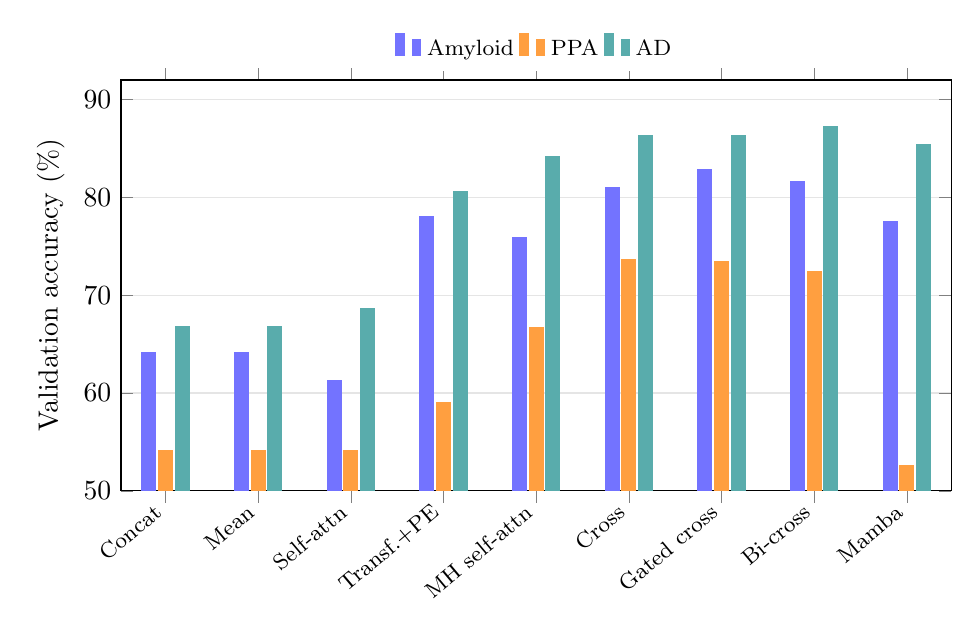
\begin{tikzpicture}
\begin{axis}[
    width=\linewidth, height=6.8cm,
    ybar=1pt, bar width=5pt,
    ymin=50, ymax=92,
    ylabel={Validation accuracy (\%)},
    ylabel near ticks,
    symbolic x coords={Concat,Mean,Self-attn,Transf.+PE,MH self-attn,Cross,Gated cross,Bi-cross,Mamba},
    xtick=data,
    x tick label style={rotate=40,anchor=east,font=\footnotesize},
    ytick={50,60,70,80,90},
    enlarge x limits=0.06,
    ymajorgrids, grid style={gray!20},
    legend style={at={(0.5,1.02)},anchor=south,legend columns=3,font=\footnotesize,draw=none},
]
\addplot[fill=blue!55,draw=blue!55] coordinates {(Concat,64.12)(Mean,64.12)(Self-attn,61.26)(Transf.+PE,78.05)(MH self-attn,75.85)(Cross,81.00)(Gated cross,82.88)(Bi-cross,81.64)(Mamba,77.49)};
\addplot[fill=orange!75,draw=orange!75] coordinates {(Concat,54.10)(Mean,54.10)(Self-attn,54.09)(Transf.+PE,59.04)(MH self-attn,66.66)(Cross,73.67)(Gated cross,73.46)(Bi-cross,72.43)(Mamba,52.57)};
\addplot[fill=teal!65,draw=teal!65] coordinates {(Concat,66.83)(Mean,66.83)(Self-attn,68.65)(Transf.+PE,80.58)(MH self-attn,84.22)(Cross,86.34)(Gated cross,86.34)(Bi-cross,87.23)(Mamba,85.40)};
\legend{Amyloid, PPA, AD}
\end{axis}
\end{tikzpicture}%
}
\caption[Fusion-family accuracy across tasks]{Validation accuracy of the fusion families on the three tasks (values from Table~\ref{tab:res_fusion}). The cross-attention family leads on every task, while Mamba's drop to chance on PPA stands out as the clearest outlier. Abbreviations: \emph{Concat}~=~concatenation, \emph{Mean}~=~element-wise mean (both non-sequential baselines); \emph{Self-attn}~=~self-attention, \emph{MH self-attn}~=~multi-head self-attention, \emph{Transf.+PE}~=~transformer with positional encoding; \emph{Cross}~=~cross-attention, \emph{Gated cross}~=~gated cross-attention, \emph{Bi-cross}~=~bidirectional cross-attention; \emph{Mamba}~=~selective state-space fusion.}
\label{fig:res_fusion_bar}
\end{figure}

This ranking is the main trend the second, independent DMHAM stack was built to check, and it survives the change of implementation. In the legacy fusion grid the cross-attention and Mamba families again lead within DMHAM (bidirectional cross-attention reaches 85.21\% validation on ADReSSo, for instance), even though DMHAM uses different encoders, a different ASR path, and a shorter training schedule. The absolute numbers diverge between the two stacks, which are not a controlled head-to-head, but the ordering of fusion families holds, and reproducing that ordering twice is the whole point of running it twice. Inference cost is not a discriminating factor among the families: with the encoder outputs precomputed and cached, every fusion variant runs in well under a millisecond per sample, so the choice is driven by accuracy alone.

\begin{table}[htbp]
\centering
\caption[Fusion-technique ablation per task]{Fusion-technique ablation per task (\texttt{res\_model}, weighted Wav2Vec~2.0 layers, no acoustic features). The first two rows (concatenation, element-wise mean) are non-sequential baselines; the remaining seven are the sequence-to-sequence fusion families of Table~\ref{tab:fusion}. Mean CV validation accuracy (\%) over seeds. Fixed per-task alignment: ADReSSo tok$\rightarrow$tok (char); amyloid word$\rightarrow$token; PPA tok$\rightarrow$tok (uniform).}
\label{tab:res_fusion}
\small
\begin{tabular}{lccc}
\toprule
 & \multicolumn{2}{c}{\textbf{SPIN}} & \textbf{ADReSSo} \\
\cmidrule(lr){2-3}\cmidrule(lr){4-4}
Fusion technique & \textbf{Amyloid} & \textbf{PPA} & AD \\
\midrule
Concatenation                 & 64.12 & 54.10 & 66.83 \\
Element-wise mean             & 64.12 & 54.10 & 66.83 \\
Self-attention                & 61.26 & 54.09 & 68.65 \\
Transformer (positional)      & 78.05 & 59.04 & 80.58 \\
Multi-head self-attention     & 75.85 & 66.66 & 84.22 \\
Cross-attention               & 81.00 & \textbf{73.67} & 86.34 \\
Gated cross-attention         & \textbf{82.88} & 73.46 & 86.34 \\
Bidirectional cross-attention & 81.64 & 72.43 & \textbf{87.23} \\
Mamba                         & 77.49 & 52.57 & 85.40 \\
\bottomrule
\end{tabular}

\vspace{2pt}
{\footnotesize Cross-attention variants dominate on every task; Mamba is competitive on English and amyloid but collapses on PPA. The concatenation and element-wise-mean baselines, and plain self-attention, stay near chance on SPIN. The two baselines also appear in the modality study (Table~\ref{tab:res_modality}); the small ADReSSo difference reflects the minimal head used there versus the full per-task recipe used here.}
\end{table}

With a fusion mechanism chosen, attention turns back to the audio branch. Two questions sit on it: whether to read the final Wav2Vec layer or a learnable mixture of all twelve, and, if a mixture, whether a single global set of weights is enough. The pooling table (Table~\ref{tab:res_wav2vec_pool}) gives a muted answer. A weighted layer stack helps ADReSSo slightly (86.64\% against 86.32\%), but on the Spanish tasks the final layer is as good or better, clearly so on PPA (74.95\% against 72.43\%). Depth, once a competent fusion is in place, buys little.

The adaptive layer mixer, evaluated only in the unified implementation, sharpens the picture. Replacing the single global weight vector with a per-utterance \emph{sample} mixer at temperature 0.1 lifts ADReSSo from 87.23\% (global mixer, uniform initialisation) to \textbf{88.16\%}, and the learned weights are interpretable: the mixer concentrates on the top layer (layer~11, weight $\approx 0.20$ against the uniform 0.083) while keeping secondary mass on the lowest layer, and it varies those weights from one utterance to the next instead of settling on a single profile (Figure~\ref{fig:res_layer_mixer}). The finer \emph{token} mixer does not improve on this, so the per-utterance sample mixer is the variant carried into the recommendation: cheap, input-conditioned, and biased toward the upper layers where lexical content concentrates.

\begin{figure}[htbp]
\centering
\resizebox{\linewidth}{!}{%
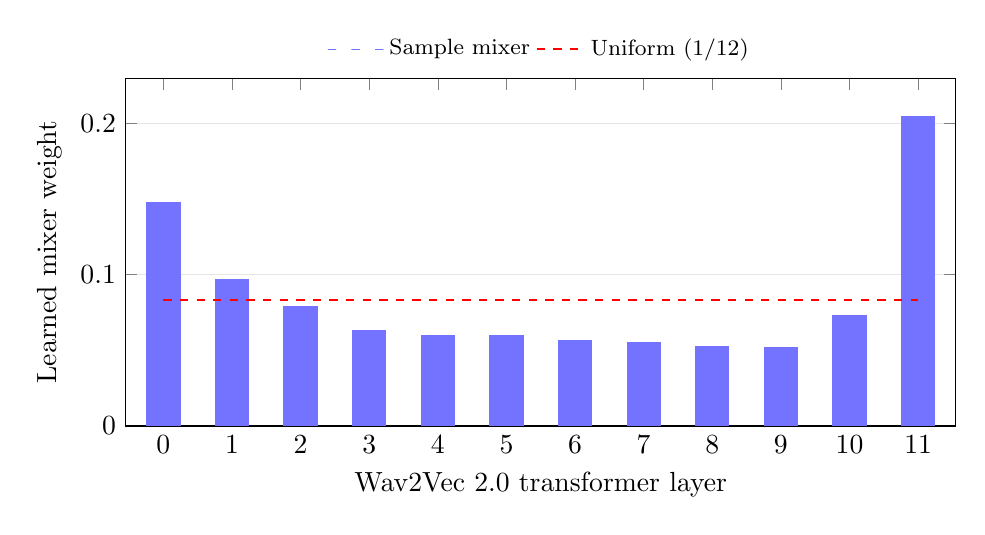
\begin{tikzpicture}
\begin{axis}[
    width=\linewidth, height=6cm,
    ylabel={Learned mixer weight},
    xlabel={Wav2Vec~2.0 transformer layer},
    symbolic x coords={0,1,2,3,4,5,6,7,8,9,10,11},
    xtick=data,
    ymin=0, ymax=0.23,
    enlarge x limits=0.05,
    ymajorgrids, grid style={gray!20},
    legend style={at={(0.5,1.02)},anchor=south,legend columns=2,font=\footnotesize,draw=none},
]
\addplot[ybar, bar width=12pt, fill=blue!55, draw=blue!55] coordinates {
    (0,0.1478)(1,0.0970)(2,0.0788)(3,0.0634)(4,0.0596)(5,0.0597)(6,0.0568)(7,0.0554)(8,0.0523)(9,0.0517)(10,0.0731)(11,0.2046)};
\addplot[red, dashed, thick, mark=none] coordinates {(0,0.0833)(11,0.0833)};
\legend{Sample mixer, Uniform ($1/12$)}
\end{axis}
\end{tikzpicture}%
}
\caption[Learned layer-mixer weights]{Learned per-layer weights of the per-utterance sample mixer on ADReSSo (seed~43, $\tau = 0.1$, twelve Wav2Vec~2.0 layers). Weight concentrates on the uppermost layer (layer~11) and, secondarily, the lowest, both well above the uniform $1/12$ baseline (dashed); the mean per-utterance spread of these weights is $0.24$.}
\label{fig:res_layer_mixer}
\end{figure}

\begin{table}[htbp]
\centering
\caption[Wav2Vec layer-pooling ablation per task]{Wav2Vec~2.0 layer-pooling ablation per task (\texttt{res\_model}, bidirectional cross-attention). \emph{Final} = last layer; \emph{weighted} = learnable 12-layer mixture. Mean CV validation accuracy (\%) over seeds. Per-task alignment: amyloid tok$\rightarrow$tok (char), PPA tok$\rightarrow$tok (uniform), ADReSSo word$\rightarrow$token.}
\label{tab:res_wav2vec_pool}
\small
\begin{tabular}{lccc}
\toprule
 & \multicolumn{2}{c}{\textbf{SPIN}} & \textbf{ADReSSo} \\
\cmidrule(lr){2-3}\cmidrule(lr){4-4}
Pooling & \textbf{Amyloid} & \textbf{PPA} & AD \\
\midrule
Final layer     & \textbf{80.75} & \textbf{74.95} & 86.32 \\
Weighted layers & 80.75 & 72.43 & \textbf{86.64} \\
\bottomrule
\end{tabular}

\vspace{2pt}
{\footnotesize Weighted layers help ADReSSo slightly; on SPIN the final layer is as good or better, especially on PPA.}
\end{table}

The next axis, audio--text alignment, is the thesis's own contribution, so it is examined under two lenses. Under the unified stable recipe (Table~\ref{tab:res_alignment}) the three schemes finish close together on all three tasks: character-proportional token-to-token is best on PPA (73.48\%), word-to-token edges amyloid (81.64\%), and on ADReSSo the two token-to-token schemes and the baseline are within a few tenths of a point. Subword alignment is therefore not a free lunch under every configuration, and that is worth stating plainly.

The larger effect appears in the configuration where it should: the legacy alignment grid on amyloid, with handcrafted features and a final-layer audio representation. There, character-proportional alignment reaches 85.72\% against 85.13\% for word-to-token, with the uniform scheme matching the baseline at 85.13\%. The proportional allocation, which gives longer subwords proportionally more of the spoken word's acoustic frames, is the one refinement that helps, and amyloid is where it helps most. Read across both lenses, the honest summary is that token-to-token alignment is a worthwhile, low-cost refinement that pays off on specific task and feature combinations rather than a universal improvement, and that the character-proportional variant is the stronger of the two proposals.

\begin{table}[htbp]
\centering
\caption[Audio--text alignment ablation per task]{Audio--text alignment ablation per task (\texttt{res\_model}, bidirectional cross-attention, weighted Wav2Vec~2.0 layers). Mean CV validation accuracy (\%) over seeds. The token$\rightarrow$token schemes are the contribution of this thesis.}
\label{tab:res_alignment}
\small
\begin{tabular}{llccc}
\toprule
 & & \multicolumn{2}{c}{\textbf{SPIN}} & \textbf{ADReSSo} \\
\cmidrule(lr){3-4}\cmidrule(lr){5-5}
Alignment & Source & \textbf{Amyloid} & \textbf{PPA} & AD \\
\midrule
word$\rightarrow$token        & CogniAlign  & \textbf{81.64} & 72.43 & \textbf{86.32} \\
tok$\rightarrow$tok (uniform) & This thesis & 79.79 & 72.43 & 86.02 \\
tok$\rightarrow$tok (char)    & This thesis & 80.75 & \textbf{73.48} & 86.02 \\
\bottomrule
\end{tabular}

\vspace{2pt}
{\footnotesize Under a stable recipe the three alignments are close on all tasks; character-proportional token$\rightarrow$token is best on PPA, while word$\rightarrow$token edges amyloid. The larger token$\rightarrow$token gain on amyloid appears in the legacy AF + final-layer stack, where the proportional scheme reaches 85.72\%.}
\end{table}

The last axis swaps the pretrained encoders one at a time (Table~\ref{tab:res_encoder}), and the outcome is firmly task-dependent. ADReSSo is best served by the original lightweight pairing of DistilBERT text with the English Wav2Vec~2.0 base encoder (86.12\%), and degrades when either is replaced, most sharply when the audio encoder switches to the multilingual XLSR-300M (80.37\%). The Spanish tasks pull the other way: XLSR-300M audio gives amyloid its best encoder result (81.40\%), and ModernBERT text helps PPA (71.70\%). The larger cross-lingual audio model earns its place precisely where the language no longer matches the English pretraining, which is the contrast the ablation was designed to expose, and a reminder that the most capable encoder is not automatically the right one once the task is fixed.

\begin{table}[htbp]
\centering
\caption[Feature-extractor single-factor ablation per task]{Feature-extractor (encoder) single-factor ablation per task (\texttt{res\_model}; fixed recipe: bidirectional cross-attention, word$\rightarrow$token, weighted Wav2Vec~2.0 + sample mixer). One component swapped per run; mean CV validation accuracy (\%) over seeds 43 and 3407.}
\label{tab:res_encoder}
\small
\begin{tabular}{lllccc}
\toprule
 & & & \multicolumn{2}{c}{\textbf{SPIN}} & \textbf{ADReSSo} \\
\cmidrule(lr){4-5}\cmidrule(lr){6-6}
Variant & Text encoder & Audio encoder & \textbf{Amyloid} & \textbf{PPA} & AD \\
\midrule
Baseline              & DistilBERT & Wav2Vec2 base-960h & 79.84 & 69.94 & \textbf{86.12} \\
Audio $\to$ XLSR      & DistilBERT & Wav2Vec2 XLSR-300M & \textbf{81.40} & 71.68 & 80.37 \\
Text $\to$ ModernBERT & ModernBERT & Wav2Vec2 base-960h & 81.36 & \textbf{71.70} & 77.38 \\
Text $\to$ BERT       & BERT-base  & Wav2Vec2 base-960h & 79.88 & 69.93 & 81.91 \\
\bottomrule
\end{tabular}

\vspace{2pt}
{\footnotesize ADReSSo favours DistilBERT + base-960h; on SPIN, XLSR-300M audio (amyloid) and ModernBERT text (PPA) slightly exceed the baseline.}
\end{table}

\subsection{Results by task}
\label{ssec:res_bytask}

Taken as a whole, the unified \texttt{res\_model} runs reproduce the main trends established on the two primitive stacks (the cross-attention family wins fusion, depth beyond the final layer adds little, and subword alignment helps narrowly and task-specifically), while adding the two studies the primitive stacks could not express cleanly: the adaptive layer mixer and the single-factor encoder swaps. The grid does not point to one winning configuration but to a different best bundle for each task, collected in Table~\ref{tab:res_best}. No two of them share the same recipe, which is the thesis's central empirical message in miniature: the best choice along each axis depends on the task, and a single configuration that wins everywhere does not exist in this grid. What the evidence supports instead is a sensible cross-task default, bidirectional cross-attention, word-to-token alignment, a weighted audio stack with the sample mixer, and handcrafted features off, that stays close to each per-task best while remaining stable across folds, seeds, and tasks. The three bundles are read out below.

\textbf{Alzheimer's disease (ADReSSo).} ADReSSo is the anchor task and the only one with an official held-out partition, so it is the one place a model is judged on a previously unseen split rather than on its own folds. The recommended configuration, bidirectional cross-attention over word-to-token-aligned streams with a weighted Wav2Vec stack refined by the per-utterance sample mixer, reaches \textbf{88.16\%} validation accuracy, obtained without leaderboard-specific tuning. The official \texttt{test-dist} partition tells a complementary story: the Mamba block edges the validation grid (88.44\%) and, run through the full-training protocol, reaches \textbf{83.10\%} on that held-out split, among the stronger challenge systems and the only configuration evaluated there. That is a genuine finding; but because the same block collapses on PPA and its ADReSSo lead is seed-sensitive, the recommendation keeps the steadier bidirectional cross-attention.

\textbf{Amyloid-$\beta$ status (SPIN).} The amyloid task recovers a fluid biomarker from forty seconds of Spanish picture description, with no official test set, so every figure is a five-fold cross-validation accuracy. It leans on the text stream (Table~\ref{tab:res_modality}), and gated cross-attention is the best plain fusion at 82.88\%. Its headline comes from the configuration the thesis contributes: character-proportional token-to-token alignment, a final-layer audio representation, bidirectional cross-attention, and the 55 handcrafted features switched on, reaching \textbf{83.90\%}. Amyloid is also where the alignment contribution shows most clearly: in the legacy handcrafted-feature and final-layer grid the proportional scheme reaches 85.72\% against 85.13\% for word-to-token, the largest of the alignment gains.

\textbf{PPA variant (SPIN).} PPA is the hardest task, a three-class problem over a small, imbalanced cohort whose fold-level accuracy is noisy, so its numbers are read as indicative rather than definitive. The best bundle, bidirectional cross-attention with uniform token-to-token alignment and a final-layer audio representation, reaches \textbf{74.95\%}. PPA is the only task that prefers audio to text as a single modality (60.03\% against 53.57\%), consistent with the motor-speech and fluency disturbances of the non-fluent variant, and the only one that punishes the wrong fusion outright, with the Mamba block falling to 52.57\%, barely above the majority class.

\begin{table}[htbp]
\centering
\caption[Best technique bundle per task]{Best technique bundle per task in the unified \texttt{res\_model} implementation. SPIN (amyloid, PPA) are Spanish, 5-fold CV validation only; ADReSSo (English) additionally reports official test-dist accuracy after full training. Mean over seeds 43 and 3407.}
\label{tab:res_best}
\small
\begin{tabular}{llcc}
\toprule
Task & Best technique stack & Val.\ acc.\ (\%) & Test acc.\ (\%) \\
\midrule
\textbf{Amyloid (SPIN)} & bicross, tok$\rightarrow$tok (char), final Wv, $+$AF & \textbf{83.90}$^{a}$ & n/a \\
\textbf{PPA (SPIN)}     & bicross, tok$\rightarrow$tok (uniform), final Wv & \textbf{74.95} & n/a \\
AD (ADReSSo, ref.)      & Mamba, word$\rightarrow$token, final Wv & 88.44 & 83.10$^{b}$ \\
\bottomrule
\end{tabular}

\vspace{2pt}
{\footnotesize $^{a}$Best single run (seed 43, lr $1.5\times10^{-5}$, dropout 0.25) with the 55-d handcrafted acoustic features; the plain-recipe gated cross-attention reaches 82.88\%. $^{b}$Official ADReSSo test-dist under the full-train protocol. Mamba tops the ADReSSo grid, but the recommended cross-task default is bidirectional cross-attention with the per-utterance sample mixer (88.16\% cross-validated validation accuracy), preferred for its stability across all three tasks rather than its single-task peak.}
\end{table}

\subsection{Error Analysis}
\label{ssec:res_error}

A detailed error analysis, including per-class confusion matrices for the three-class PPA task and an inspection of misclassified ADReSSo and amyloid cases, is left as future work. The present study reports point-estimate accuracies without confusion-level breakdowns or significance testing; characterising systematic failure modes, for example confusion between the logopenic and non-fluent PPA variants or the influence of ASR transcription errors on the text stream, would require the per-sample prediction logs and is identified here as a direction for subsequent analysis rather than reported with fabricated figures.


%%% BDGET %%%
\clearpage

\section{Budget}
% TODO: Write budget — compute/GPU hours, software, personnel cost as applicable.

%%% ENVIRONMENT %%%
\clearpage

\section[Environment Impact (Optional)]{{Environment Impact (Optional)}}

% TODO: Optional — describe environmental impact (e.g. training energy /
% carbon footprint of the GPU experiments) or remove the section.

%%% CONCLUSION AND FUTURE %%%
\clearpage
\section{Conclusions and Future Development}
\label{sec:conclusions}

% TODO: Write conclusions — summary of findings, recommended architecture
% synthesis, limitations, and future work. Do not leave template text in body.

%%% BIBLIOGRAPHY %%%
\newpage

\medskip
\bibliographystyle{unsrt}
\bibliography{bibliography}

%%% ANNEX %%%
\clearpage
\newpage

\begin{appendices}

% TODO: Optional appendices, or remove the appendices block.

\end{appendices}

\end{document}